\documentclass[journal, a4paper]{IEEEtran}
\usepackage{graphicx}
\usepackage{hyperref}
\bibliography{googlenet}
% some very useful LaTeX packages include:

%\usepackage{cite}      % Written by Donald Arseneau
                        % V1.6 and later of IEEEtran pre-defines the format
                        % of the cite.sty package \cite{} output to follow
                        % that of IEEE. Loading the cite package will
                        % result in citation numbers being automatically
                        % sorted and properly "ranged". i.e.,
                        % [1], [9], [2], [7], [5], [6]
                        % (without using cite.sty)
                        % will become:
                        % [1], [2], [5]--[7], [9] (using cite.sty)
                        % cite.sty's \cite will automatically add leading
                        % space, if needed. Use cite.sty's noadjust option
                        % (cite.sty V3.8 and later) if you want to turn this
                        % off. cite.sty is already installed on most LaTeX
                        % systems. The latest version can be obtained at:
                        % http://www.ctan.org/tex-archive/macros/latex/contrib/supported/cite/

\usepackage{graphicx}   % Written by David Carlisle and Sebastian Rahtz
                        % Required if you want graphics, photos, etc.
                        % graphicx.sty is already installed on most LaTeX
                        % systems. The latest version and documentation can
                        % be obtained at:
                        % http://www.ctan.org/tex-archive/macros/latex/required/graphics/
                        % Another good source of documentation is "Using
                        % Imported Graphics in LaTeX2e" by Keith Reckdahl
                        % which can be found as esplatex.ps and epslatex.pdf
                        % at: http://www.ctan.org/tex-archive/info/

%\usepackage{psfrag}    % Written by Craig Barratt, Michael C. Grant,
                        % and David Carlisle
                        % This package allows you to substitute LaTeX
                        % commands for text in imported EPS graphic files.
                        % In this way, LaTeX symbols can be placed into
                        % graphics that have been generated by other
                        % applications. You must use latex->dvips->ps2pdf
                        % workflow (not direct pdf output from pdflatex) if
                        % you wish to use this capability because it works
                        % via some PostScript tricks. Alternatively, the
                        % graphics could be processed as separate files via
                        % psfrag and dvips, then converted to PDF for
                        % inclusion in the main file which uses pdflatex.
                        % Docs are in "The PSfrag System" by Michael C. Grant
                        % and David Carlisle. There is also some information
                        % about using psfrag in "Using Imported Graphics in
                        % LaTeX2e" by Keith Reckdahl which documents the
                        % graphicx package (see above). The psfrag package
                        % and documentation can be obtained at:
                        % http://www.ctan.org/tex-archive/macros/latex/contrib/supported/psfrag/

%\usepackage{subfigure} % Written by Steven Douglas Cochran
                        % This package makes it easy to put subfigures
                        % in your figures. i.e., "figure 1a and 1b"
                        % Docs are in "Using Imported Graphics in LaTeX2e"
                        % by Keith Reckdahl which also documents the graphicx
                        % package (see above). subfigure.sty is already
                        % installed on most LaTeX systems. The latest version
                        % and documentation can be obtained at:
                        % http://www.ctan.org/tex-archive/macros/latex/contrib/supported/subfigure/

\usepackage{url}        % Written by Donald Arseneau
                        % Provides better support for handling and breaking
                        % URLs. url.sty is already installed on most LaTeX
                        % systems. The latest version can be obtained at:
                        % http://www.ctan.org/tex-archive/macros/latex/contrib/other/misc/
                        % Read the url.sty source comments for usage information.

%\usepackage{stfloats}  % Written by Sigitas Tolusis
                        % Gives LaTeX2e the ability to do double column
                        % floats at the bottom of the page as well as the top.
                        % (e.g., "\begin{figure*}[!b]" is not normally
                        % possible in LaTeX2e). This is an invasive package
                        % which rewrites many portions of the LaTeX2e output
                        % routines. It may not work with other packages that
                        % modify the LaTeX2e output routine and/or with other
                        % versions of LaTeX. The latest version and
                        % documentation can be obtained at:
                        % http://www.ctan.org/tex-archive/macros/latex/contrib/supported/sttools/
                        % Documentation is contained in the stfloats.sty
                        % comments as well as in the presfull.pdf file.
                        % Do not use the stfloats baselinefloat ability as
                        % IEEE does not allow \baselineskip to stretch.
                        % Authors submitting work to the IEEE should note
                        % that IEEE rarely uses double column equations and
                        % that authors should try to avoid such use.
                        % Do not be tempted to use the cuted.sty or
                        % midfloat.sty package (by the same author) as IEEE
                        % does not format its papers in such ways.

\usepackage{amsmath}    % From the American Mathematical Society
                        % A popular package that provides many helpful commands
                        % for dealing with mathematics. Note that the AMSmath
                        % package sets \interdisplaylinepenalty to 10000 thus
                        % preventing page breaks from occurring within multiline
                        % equations. Use:
%\interdisplaylinepenalty=2500
                        % after loading amsmath to restore such page breaks
                        % as IEEEtran.cls normally does. amsmath.sty is already
                        % installed on most LaTeX systems. The latest version
                        % and documentation can be obtained at:
                        % http://www.ctan.org/tex-archive/macros/latex/required/amslatex/math/



% Other popular packages for formatting tables and equations include:

%\usepackage{array}
% Frank Mittelbach's and David Carlisle's array.sty which improves the
% LaTeX2e array and tabular environments to provide better appearances and
% additional user controls. array.sty is already installed on most systems.
% The latest version and documentation can be obtained at:
% http://www.ctan.org/tex-archive/macros/latex/required/tools/

% V1.6 of IEEEtran contains the IEEEeqnarray family of commands that can
% be used to generate multiline equations as well as matrices, tables, etc.

% Also of notable interest:
% Scott Pakin's eqparbox package for creating (automatically sized) equal
% width boxes. Available:
% http://www.ctan.org/tex-archive/macros/latex/contrib/supported/eqparbox/

% *** Do not adjust lengths that control margins, column widths, etc. ***
% *** Do not use packages that alter fonts (such as pslatex).         ***
% There should be no need to do such things with IEEEtran.cls V1.6 and later.
\usepackage{fancyhdr}
\pagestyle{fancy}
\fancyfoot{}
\fancyfoot[RO, LE] {\thepage}

\lfoot{\footnotesize \href{https://github.com/tpsatish95/pokemon-vqa}{\textsc{Pok\'emon VQA Code:} https://github.com/tpsatish95/pokemon-vqa}}

% Your document starts here!
\begin{document}

% Define document title and author
	\title{Visual Question Answering}
	\author{Satish Palaniappan, Ayush Agarwal, Sonakshi Grover

	\thanks{Advisor: Dr Greg Hager, Mandell Bellmore Professor of Computer Science, Johns Hopkins University. \newline 
	\textsc{Pok\'emon VQA Code:} https://github.com/tpsatish95/pokemon-vqa}}
	%\markboth{Hauptseminar Digitale Kommunikationssysteme}{}
	\maketitle

% Write abstract here
\begin{abstract}
	Recent advances in deep learning have provided a platform to accomplish tasks involving multimodal learning. Visual Question Answering (VQA) is one such recent problem in computer vision and natural language processing. In VQA, an algorithm needs to answer text-based questions about images. These questions require methods to understand vision, language and common-sense domain knowledge to output an reasonable answer. In this project, we attempt to leverage transfer learning to solve the VQA problem in the domain of the popular anime series, Pok\'emon. In addition, we provide an insight into the domain-specific requirements for a successful transfer. Our method is able to obtain a test accuracy of 65\% on some fixed basic questions applied to Pok\'emon battle scene images. While there is no available state of the art in the domain, we observe that we are able to match the SOTA performance on the baseline when we work with our dataset. 
\end{abstract}

% Each section begins with a \section{title} command
\section{Introduction}
	% \PARstart{}{} creates a tall first letter for this first paragraph
	The emergence of many successful deep learning pipelines to facilitate multiple tasks learned end to end has led to the recent spurt of work in Visual Question Answering. The problem statement involves the development of an algorithm which can take into input an image and a textual question and outputs an answer to the question based on the visual features from the input image. Our system considers the first 150 Pok\'emon (Kanto Region) and some sample questions our Pok\'emon VQA model will try to answer are:
	\begin{itemize}
	    \item Q: What Pok\'emon is there in the image? \\A: Pikachu.
	    \item Q: What attack is being performed by Pikachu? \\A: Thunderbolt
	    \item Q: What type of Pok\'emon is Pikachu? \\A: Electric
	\end{itemize}
	    
	In Section 2, we start by discussing some related work in the field of VQA along with our insights we present by reproducing their results on the baseline. In section 3, we proceed with explaining the nuances of our dataset creation pipeline, where we detail the methods to construct three separate databases: Pok\'emons, Battle scene attacks and Questions based on Pokemon moves and statistics, which will be mapped together to generate the dataset for the VQA model.
    Section 4 will explore our train and transfer paradigm, where we describe the architecture and parameters of the model used to train on our dataset from scratch. Finally, we look at the results obtained on different parameters we experimented with in Section 5.
    \begin{figure}[ht]
    \caption{Workflow of our project pipeline}
\centering
    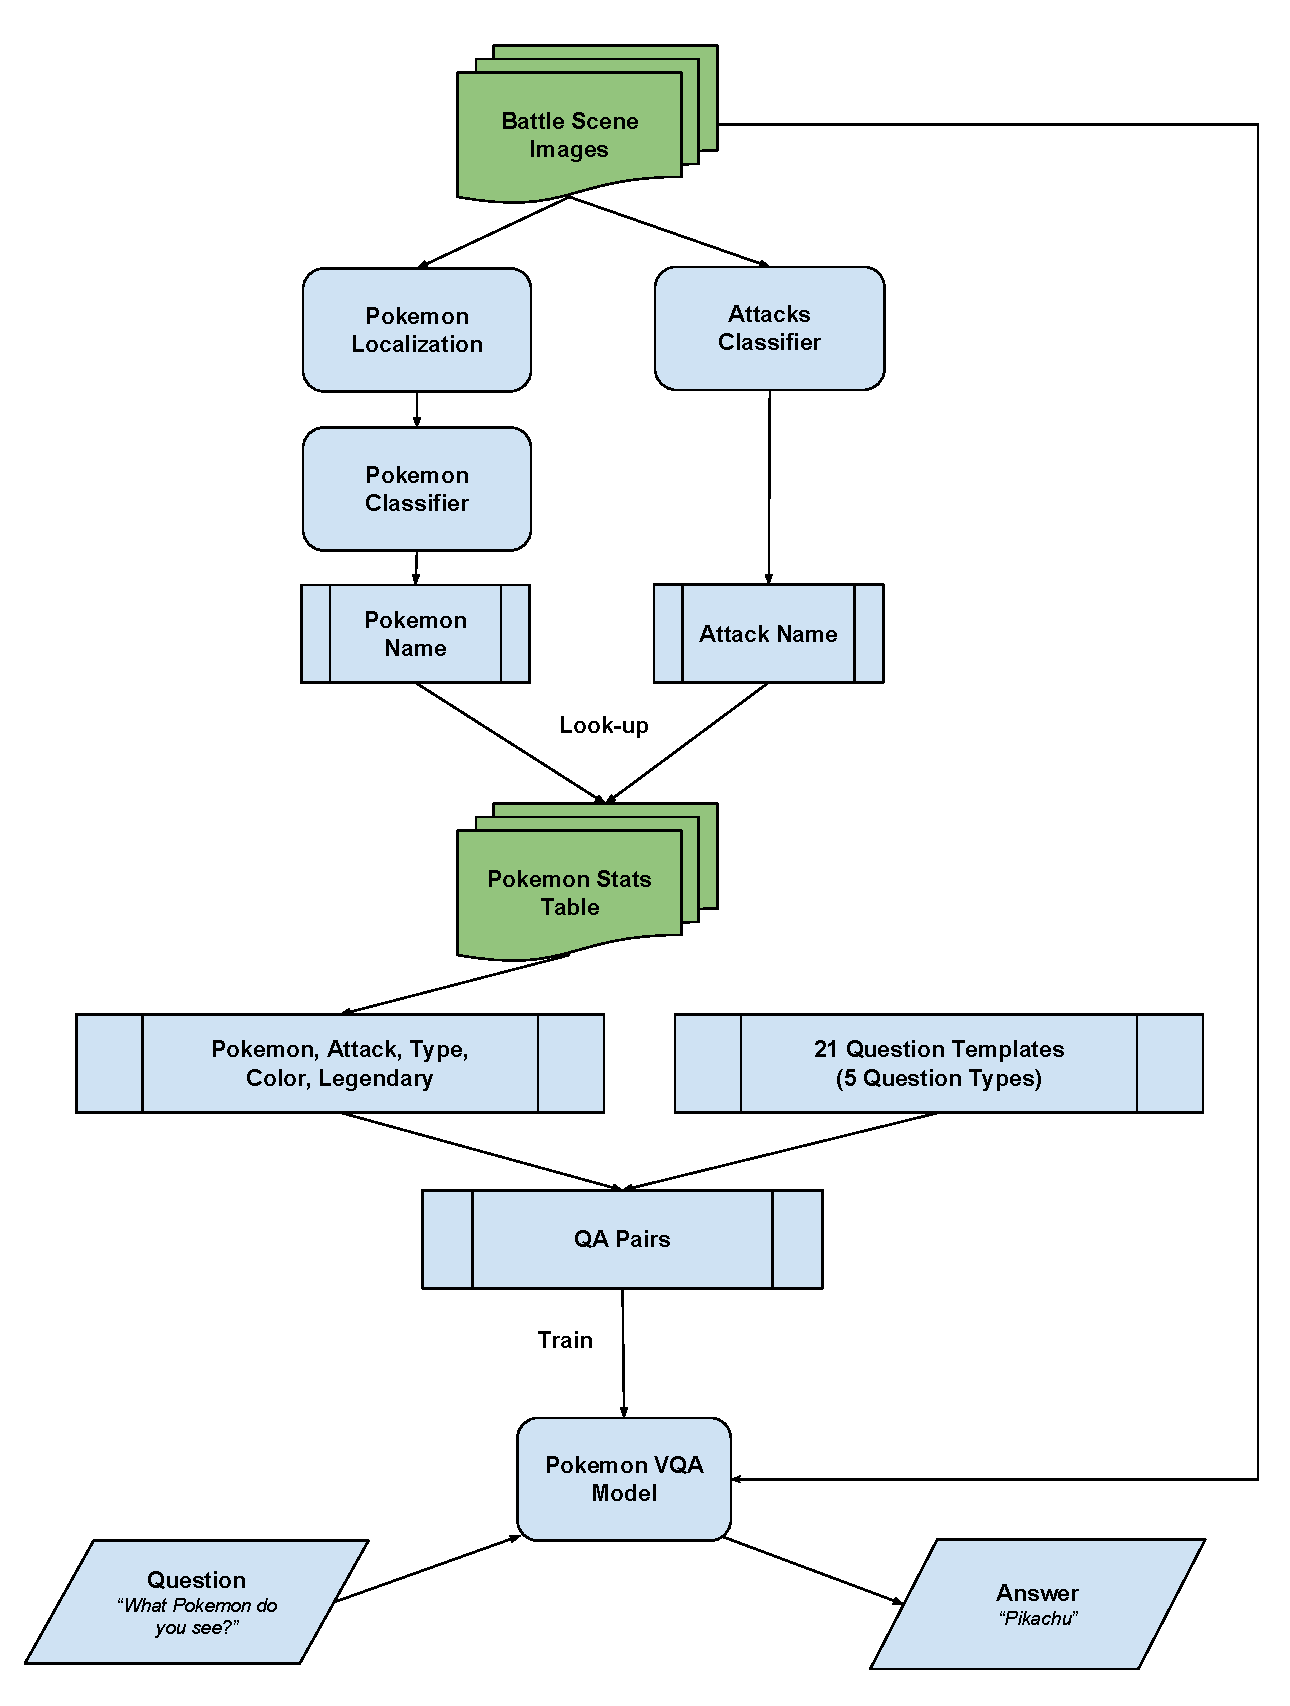
\includegraphics[scale = 0.6, width=7cm, height=9cm]{VQA_Pokemon_Workflow.pdf}
    \end{figure}

% Main Part
\section{Related Work}
	We identified $3-$4 implmentations of the VQA state of the art which we attempted to reproduce their results with our available computing resources. Jiang et. al. \cite{PYTHIA} introduced the Pythia which was the winning entry from Facebook AI Research (FAIR)'s A-STAR team to the VQA Challenge 2018. They make important changes to tune better hyperparameters and make a modular code for the bottom up- top down VQA model (Anderson et. al. \cite{BOTTOMUP}). Since each training run takes over a day, not mentioning the RAM needed to store huge Resnet-152 based features, unfortunately even with the increased compute power from the cloud credits, we were unable to reproduce the baseline from scratch. We thus moved to more optimized and smaller versions of the bottom up top down VQA model (available at \cite{VQA1}, \cite{VQA2}). These involved extracting the image features from a smaller VGG-19 structure and then training an end to end network by combining the image features with textual features from the question mappings (obtained from a separate LSTM model) and applying a multi-layer perceptron on the combined features. 
	\newline
	\textit{Note: these papers already had implementations with pre-trained weights available and hence it was merely a matter of tweaking this code a bit to get it to work on GCP and generate results on our dataset}

\section{Dataset}
The dataset creation for the Pok\'emon VQA problem involves the following 4 steps: \\

\begin{itemize}
    \item Build a region proposal algorithm to locate Pok\'emon in battle scenes.
    \item Build a Pok\'emon and Attacks classifier to label the battle scenes.
    \item Construct questions using the Pok\'emon stats dataset.
    \item Map questions to battle scene images using the Pok\'emon \& Attack labels.
\end{itemize}

\textbf{Step 1:} Build a region proposal algorithm to locate Pok\'emon in battle scenes:

In this step, first we used a region proposal algorithm called Selective Search\cite{SELECTIVE SEARCH} \cite{SELECTIVE SEARCH CODE} to generate the first set of candidate region proposals. Selective search is an object detection algorithm which proposes various regions in an image that are highly probable to contain an object in them. Selective Search parameters used (best): \textbf{Scale - 350, 450, 500; Sigma - 0.8; Min. Size - 30, 60, 120, Min Area - 2000}.

But, these initial candidate region proposals are large in number, in order to reduce them quantitatively and improve them qualitatively, we came up with some Region Proposal Filtering methods like: \textbf{Merge Concentric Proposals, Contained Box Removal, Draw Super Box}. Fig. 2 shows a sample, after applying both of the above operations:

 \begin{figure}[ht]
    \caption{Sample image obtained after Selective Search and Region Proposal Filtering}
\centering
 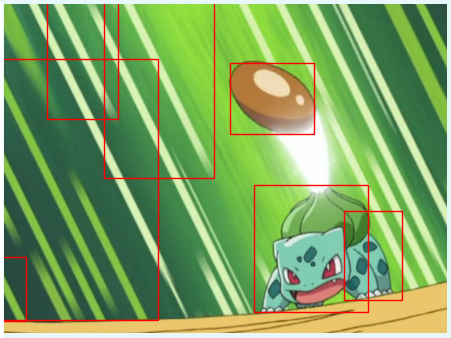
\includegraphics[scale = 0.3, width=9cm]{ppo.png}
    \end{figure}

Now, from these highly probable candidates, in order to get the exact regions where the Pok\'emon are located. We ended up building a very simple 3 class classifier, called the Pok\'emon/Part/Other classifier. This used \textbf{GoogLeNet Inception V1} \cite{googlenet} architecture with the weights transferred from ImageNet \cite{IMAGENET}. \textbf{Accuracy: 74.9\%}. The base dataset was generated by hand-labeling and had 3639 images in total with 3 classes and the dataset was balanced with 80\% for train and 20\% for test, which looks like Fig. 3.

\begin{figure}[ht]
    \caption{Sample images from the Pok\'emon/Part/Other (top to bottom) Dataset}
\centering
 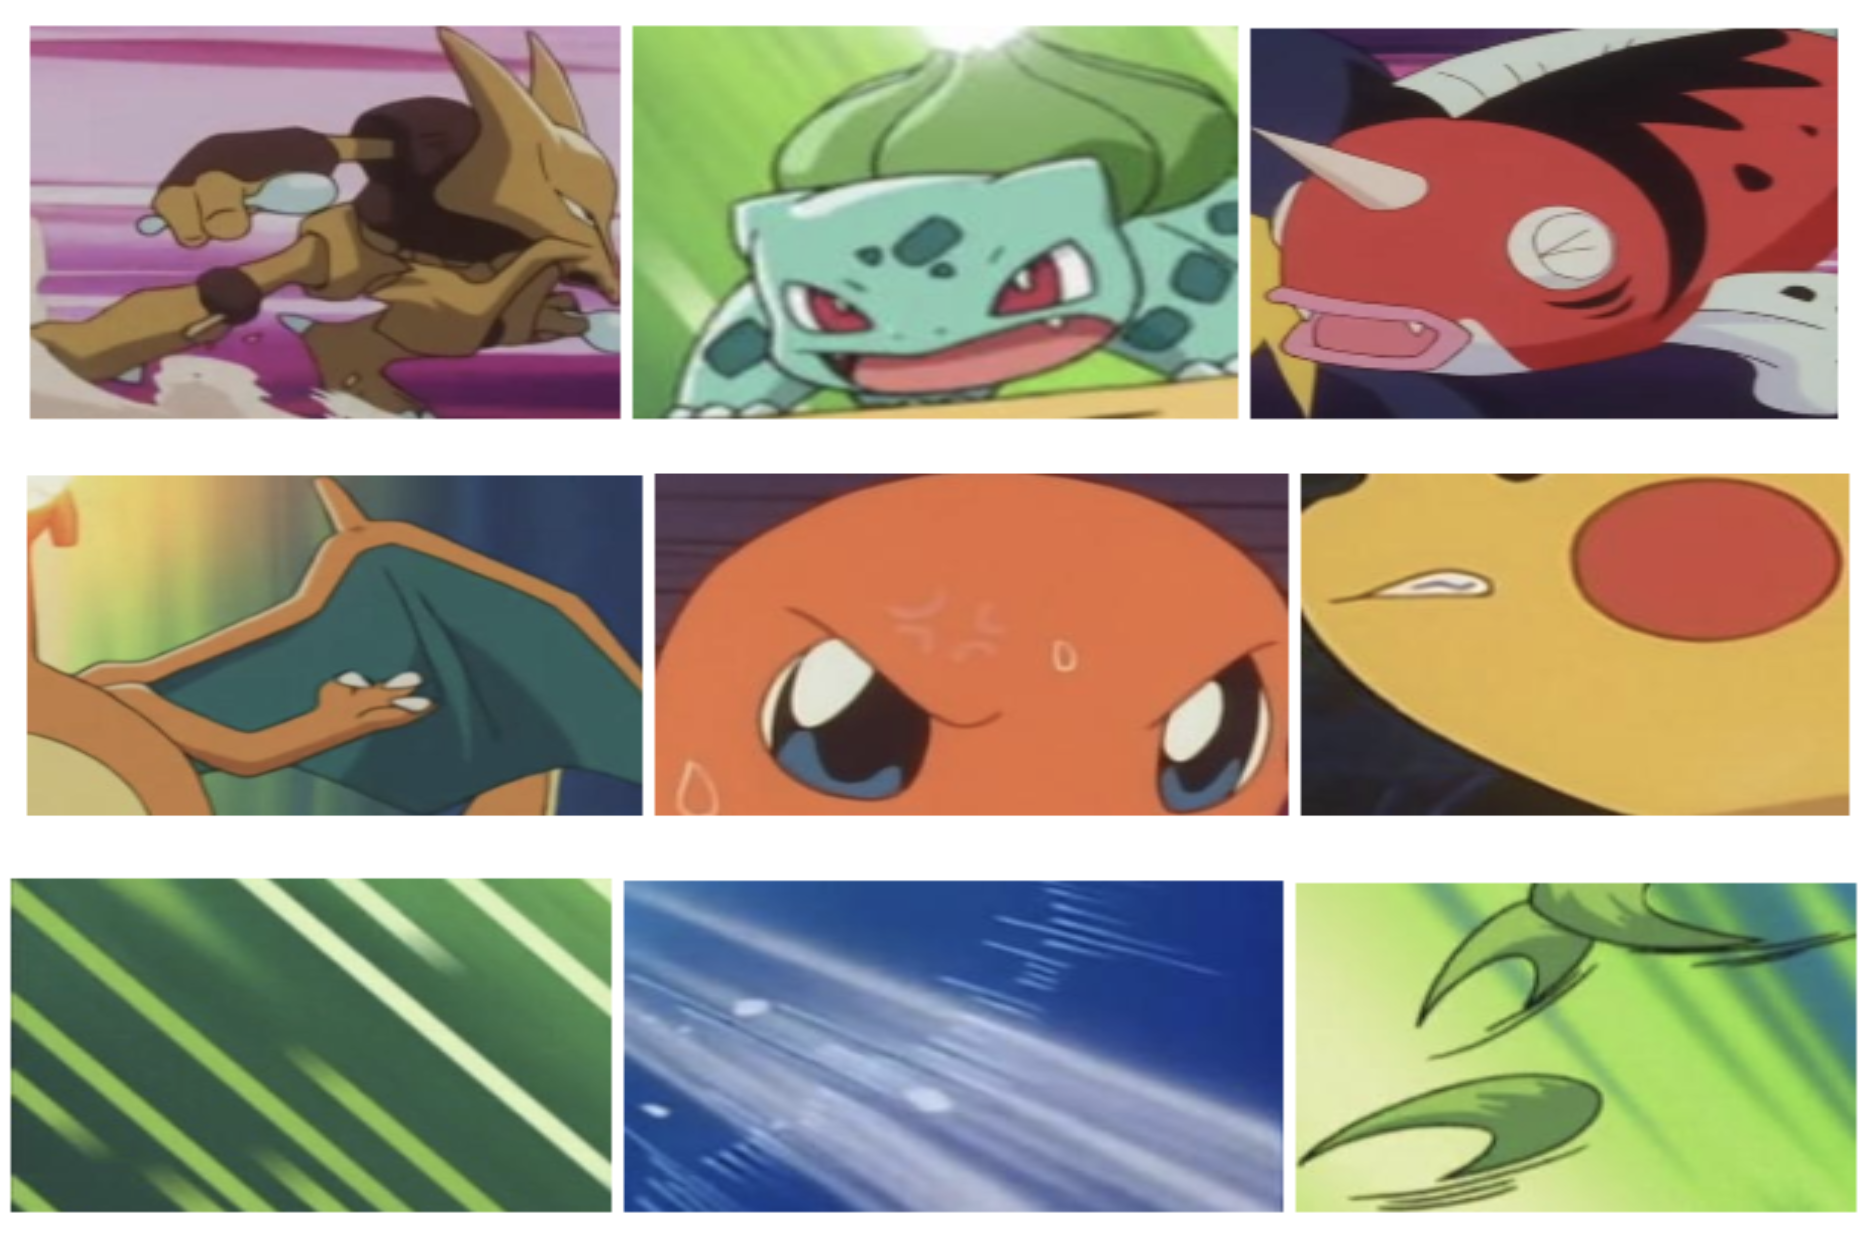
\includegraphics[scale = 0.6, width=9cm]{ppo1.png}
    \end{figure}

Using the above-described classifier, each of the current candidate region proposals were classified. Once we know the kind of each region we have in hand, we used basic rules like merging overlapping \textbf{Pok\'emon} and \textbf{Part} regions while subtracting the overlapping \textbf{Other} regions from them to arrive at the final Pok\'emon only regions as shown in Fig. 4.

\begin{figure}[ht]
    \caption{Finalized region proposal locating the Pok\'emon}
\centering
 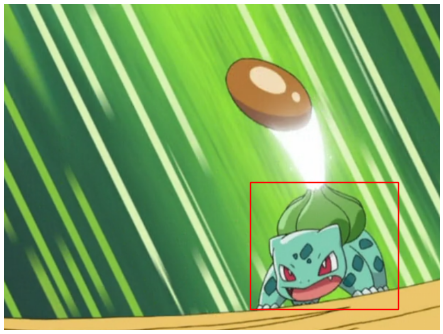
\includegraphics[scale = 0.6, width=9cm]{ppo2.png}
    \end{figure}

\textbf{Step 2:} Build a Pok\'emon and Attacks classifier to label the battle scenes:

\textbf{Pok\'emon Classifier:} Given that we have extracted the Pok\'emon only regions from the battle image, the next step would be to classify these Pok\'emon. We again used a \textbf{GoogLeNet Inception V1} architecture pre-trained on the ImageNet dataset for building this 150 class classifier. We pulled the base dataset for this from Kaggle \cite{KAGGLE} and Bulbapedia \cite{BULBAPEDIA}, and then augmented them by applying random image transforms such as: rotation, scaling, translation, swirl, shear, horizontal/veritical flips, and blur. Then this augmented dataset was superimposed on typical battle scene backgrounds like the ones found \href{https://drive.google.com/drive/folders/1LhRDXpVSsk9nHymrT8Dy9LQcLmGcC546}{here}. This dataset had a total of 134508 images and 150 classes, which were generated from just 1076 base Pok\'emon images. These images were then augmented using the techniques mentioned above to 5x, which is 5380 images. Then these augmented images were imposed on 25 distinct background images to get the final 134508 images, with a 70-30 train-test split. See dataset sample Fig. 5.

\begin{figure}[ht]
    \caption{Pok\'emon Classifier Dataset Sample}
\centering
 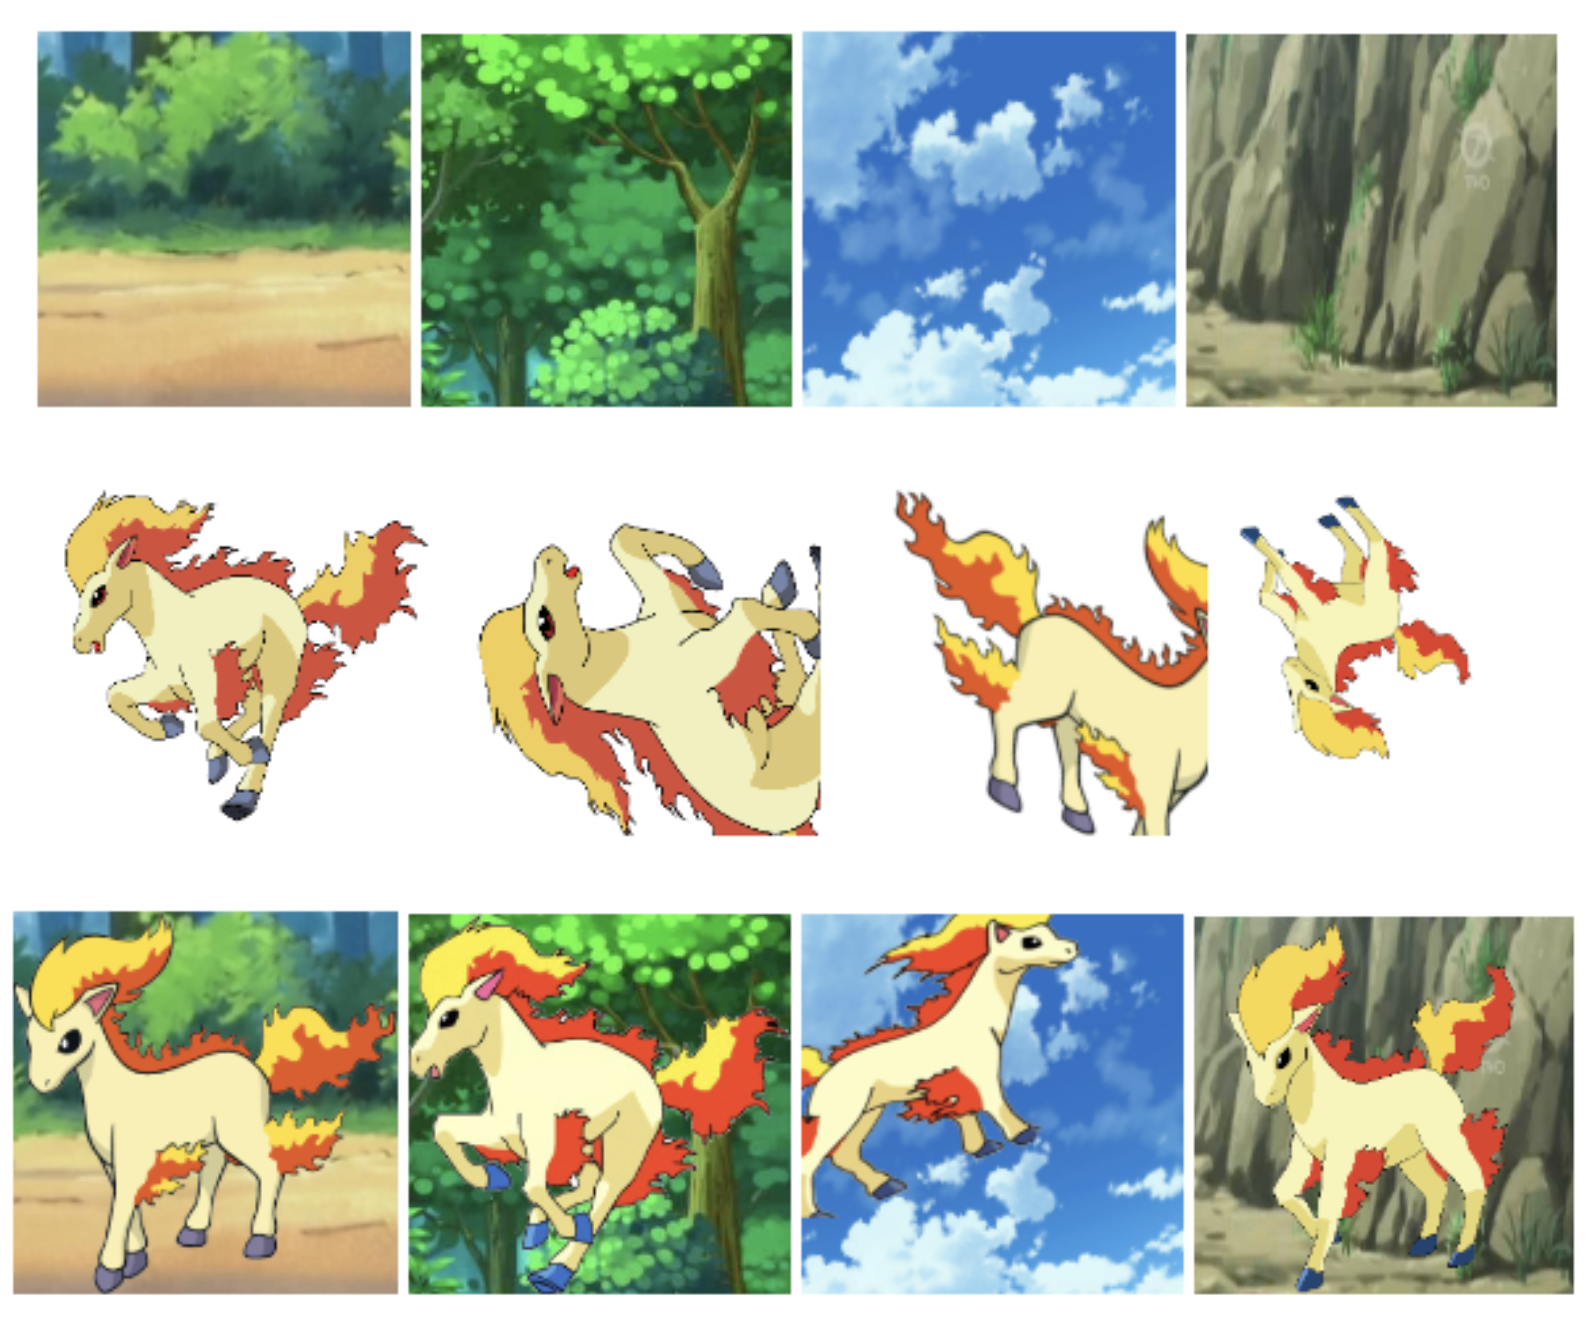
\includegraphics[scale = 0.6, width=9cm]{poke_data.png}
    \end{figure}

This model achieved a Top-1 accuracy of \textbf{91.16\%} and Top-5 accuracy of \textbf{98.03\%} with Backgrounded and Augmented dataset, while it achieves only Top-1 accuracy of \textbf{85.39\%} and Top-5 accuracy of \textbf{96.43\%} with just the Augmented dataset. The Hyperparameter configuration used are shown in Fig 6. Some sample results of the classifier are shown in Fig 7.

\begin{figure}[ht]
    \caption{GoogLeNet Inception V1 Best Hyper Paramter Configuration}
\centering
 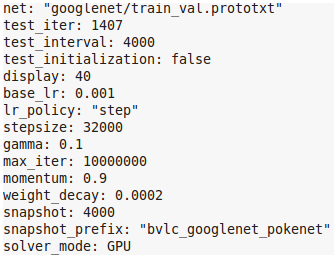
\includegraphics[scale = 0.6, width=9cm]{cnn4.png}
    \end{figure}

\begin{figure}[ht]
    \caption{Pok\'emon Classifier Top-5 results}
\centering
 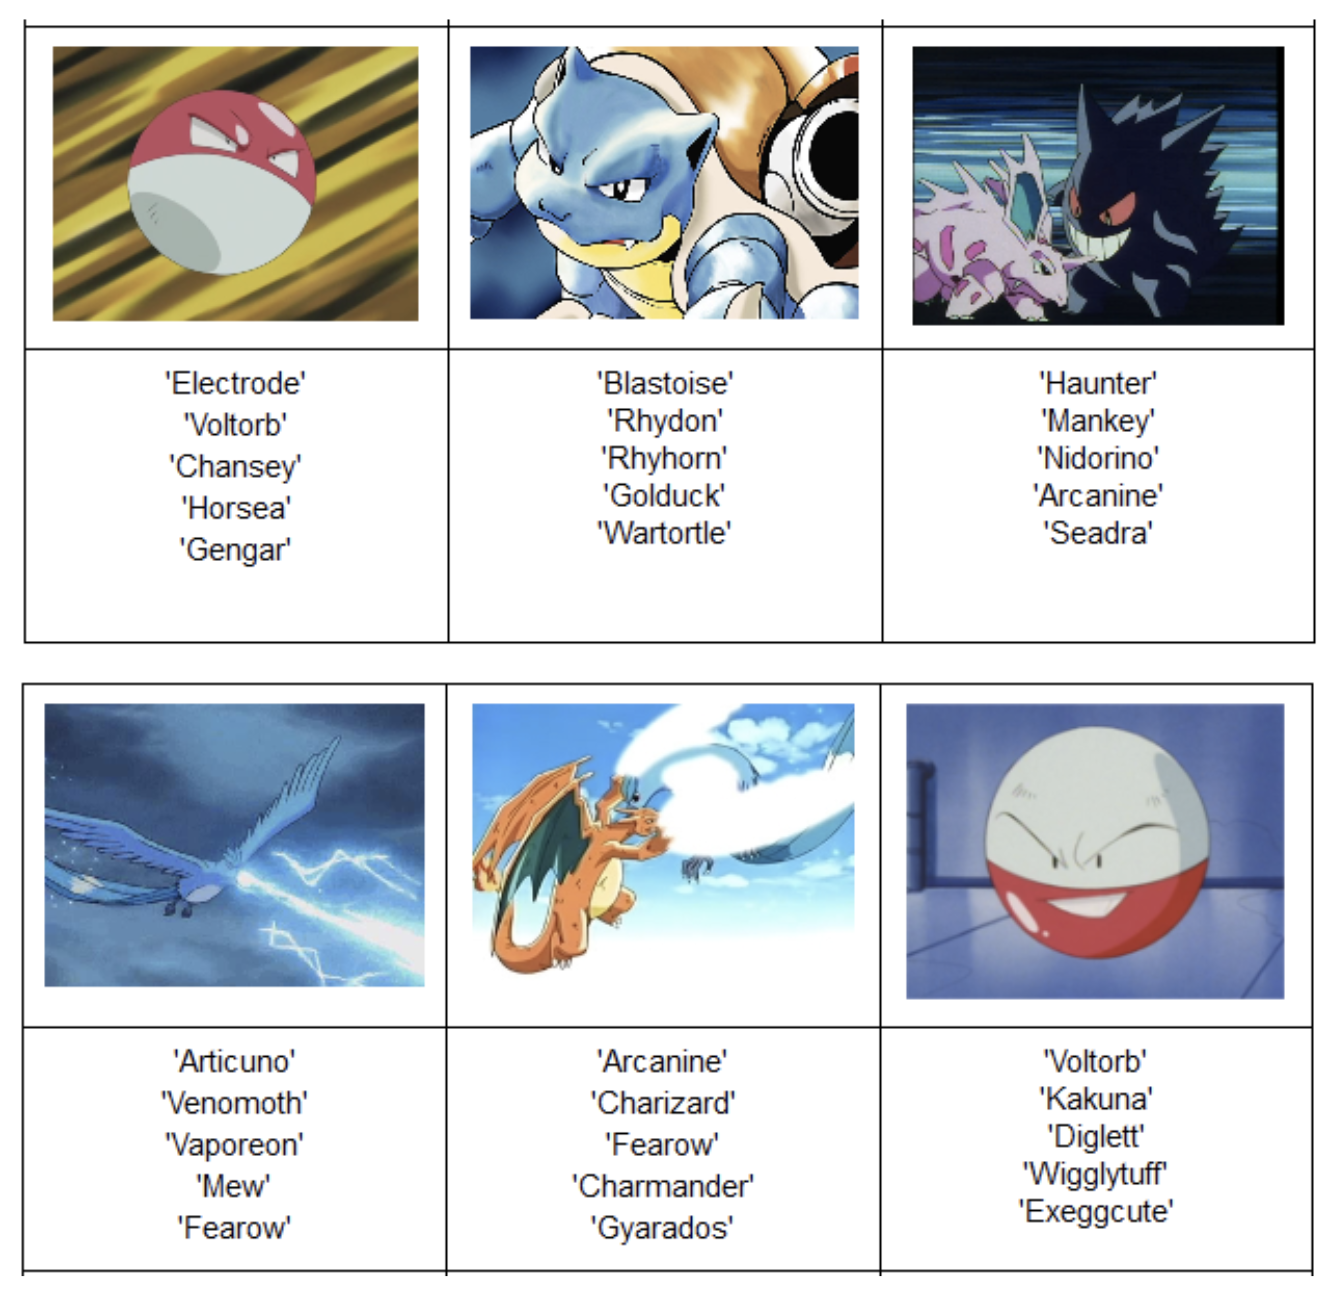
\includegraphics[scale = 0.6, width=9cm]{poke_results.png}
    \end{figure}

\textbf{Attacks classifier:} For this classifier we will again be using the \textbf{GoogLeNet Inception V1} architecture, but this time around, we do not need the Pok\'emon regions as attack classification is much similar to a scene classification problem than an object classification problem. So, we used a GoogLeNet pre-trained on the \textbf{MIT Places 205}\cite{MIT 205 PLACES} dataset to transfer learn this attacks classifier. The attacks dataset was crawled from Bulbapedia \cite{BULBAPEDIA} and Pok\'emon Wikia\cite{WIKIA}. Which was then augmented using similar techniques as discussed above to get 21188 images with 144 attack classes finally, which was split into 70-30 for train-test. Some attack samples (Thunderbolt, Flamethrower, Water Gun, etc) can be found in Fig. 8, there are 144 attacks in total.

\begin{figure}[ht]
    \caption{Attacks Classifier Dataset}
\centering
 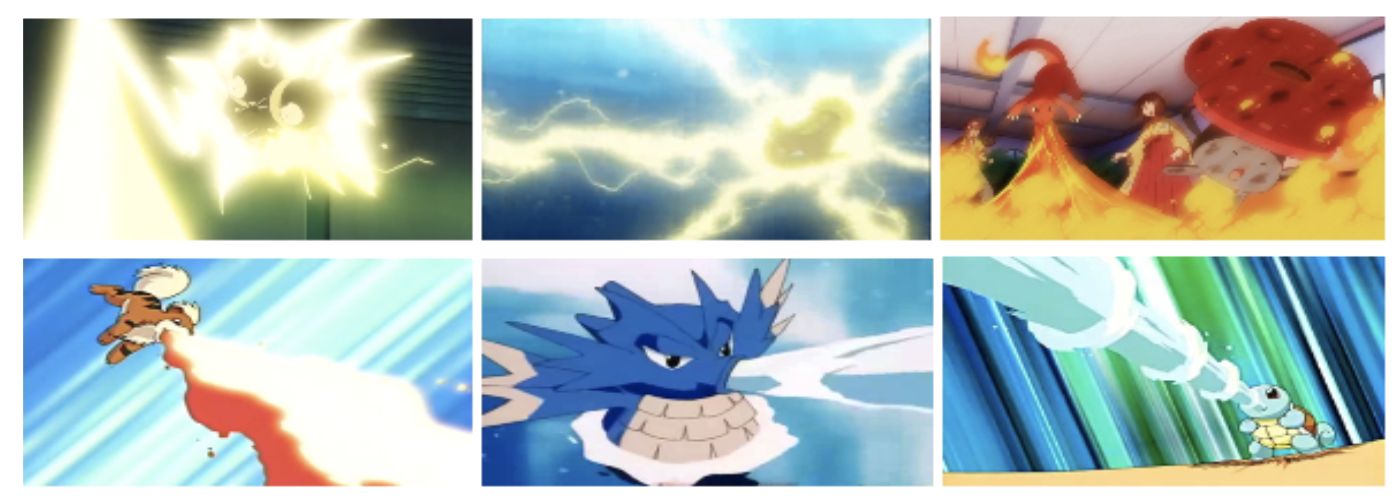
\includegraphics[scale = 0.6, width=9cm]{attack.png}
\end{figure}

We obtained a \textbf{88\% top-5 accuracy and a 55\% top-1 accuracy} for this Attacks Classifier. Though these accuracies are low, using restricted Pokemon-Attacks mappings we boosted the accuracy of these classsifiers based on the Pok\'emon data we figured out. Because a given Pok\'emon can only perform 10 attacks and not all 144 of them. Fig 9. Shows some sample attack classifier results.

\begin{figure}[ht]
    \caption{Attacks Classifier Results}
\centering
 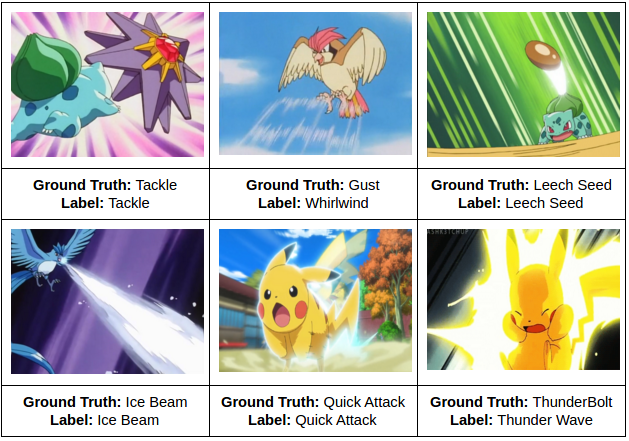
\includegraphics[scale = 0.6, width=9cm]{attackresult.png}
\end{figure}

\textbf{Step 3:} Construct questions using the Pok\'emon stats dataset:

Before we see how we gathered data to construct questions, lets see how we built the battle scenes dataset, which will essentially be the image input to our VQA model. We crawled Bulbapedia for battle scene images and got 1511 images in total which were split into 80-20 for train-test. Once we got these input VQA images, we then feed these into the Pok\'emon and Attacks Classifier designed in Step 2, to get the Pok\'emon present and Attack being performed information for a battle scene. Then we use this to lookup the Pok\'emon Stats \cite{STATS} table and get more information like the Pok\'emon's type, color and legendary information for generating more QA pairs as described in Step 4.

\textbf{Step 4:} Map questions to battle scene images using the Pok\'emon \& Attack labels:\\
Once we process the input battle scene images as in Step 3, we will have sets of [Battle Scene Image, Pok\'emon, Attack, Color, Type, Is Legendary] for each of the 1511 images. Then we generated 21 questions for each of these images with 5 distinct types (as listed below) and other 16 questions were equivalent/paraphrased versions of these:

\begin{enumerate}
    \item What pokemon is there in the image?
    \item What attack is being performed by the pokemon?
    \item What type of pokemon is it?
    \item Is the pokemon legendary?
    \item What is the color of the pokemon in the image?
\end{enumerate}
               
So, we got the Pok\'emon and attack names (from step 2), Pok\'emon color, type and legendary data (from step 3) and then basically now are doing a cross product of all 21 questions for each of the 1511 battle scene images, to generate the 31,731 QA pairs with a 70-30 split for train-test.

Before feeding these QA pairs to the network we preprocess it. We tokenize the sentences and map each token(word) to an id. The vocabulary size is 37 words. We have 304 possible answers including the different attacks, colors and Pok\'emons. After this, we create a JSON object for every QA pair wherein the keys of JSON object comprises of question ID, image path, question and answer.

\section{Model Architecture and Training}
	We finally used the model available at \cite{VQA_MODEL}. The model structure involves looking at the image input, reads a question and comes up with an answer and an attention heatmap denoting the most important regions in the image it observed to output the answer. The model also supports referring the image repeatedly with intermediate attention maps before producing the final answer. 
    
    Compared to models that simply combine the question
vector and the global image vector, attention models
construct a more informative query vector at each stage since higher weights are put on the visual regions that are more relevant to the question. Each attention layer extracts more fine-grained visual attention information
for answer prediction.

For the kth attention layer, the following is the formulation of these stacked attention networks:
\begin{equation}
h_A^k = tanh (W_{i,A}^k*v_i + (W_{Q,A}^k*u^{k-1} + b_a^k))
\end{equation}
\begin{equation}
p_i^k = softmax(W_{p}^k*h_A^k)
\end{equation}
The first equation is the activation generated on combining the image features obtained from the VGG 19 network and the question vector. The second equation applies a softmax function to generate the attention map over the image.
Then the aggregated image
feature vector is added to the previous query vector to form a new query vector:
\begin{equation}
{v'}_i^k = {\sum\limits_i}p_i^k * v_i
\end{equation}
\begin{equation}
{u}^k = {v'}_i^k + u^{k-1}
\end{equation}
This vector is propagated through the network until the final answer is produced. 
\vspace{-5mm}
\begin{figure}[ht]
    \caption{Diagram summary of the model from the paper}
\centering
 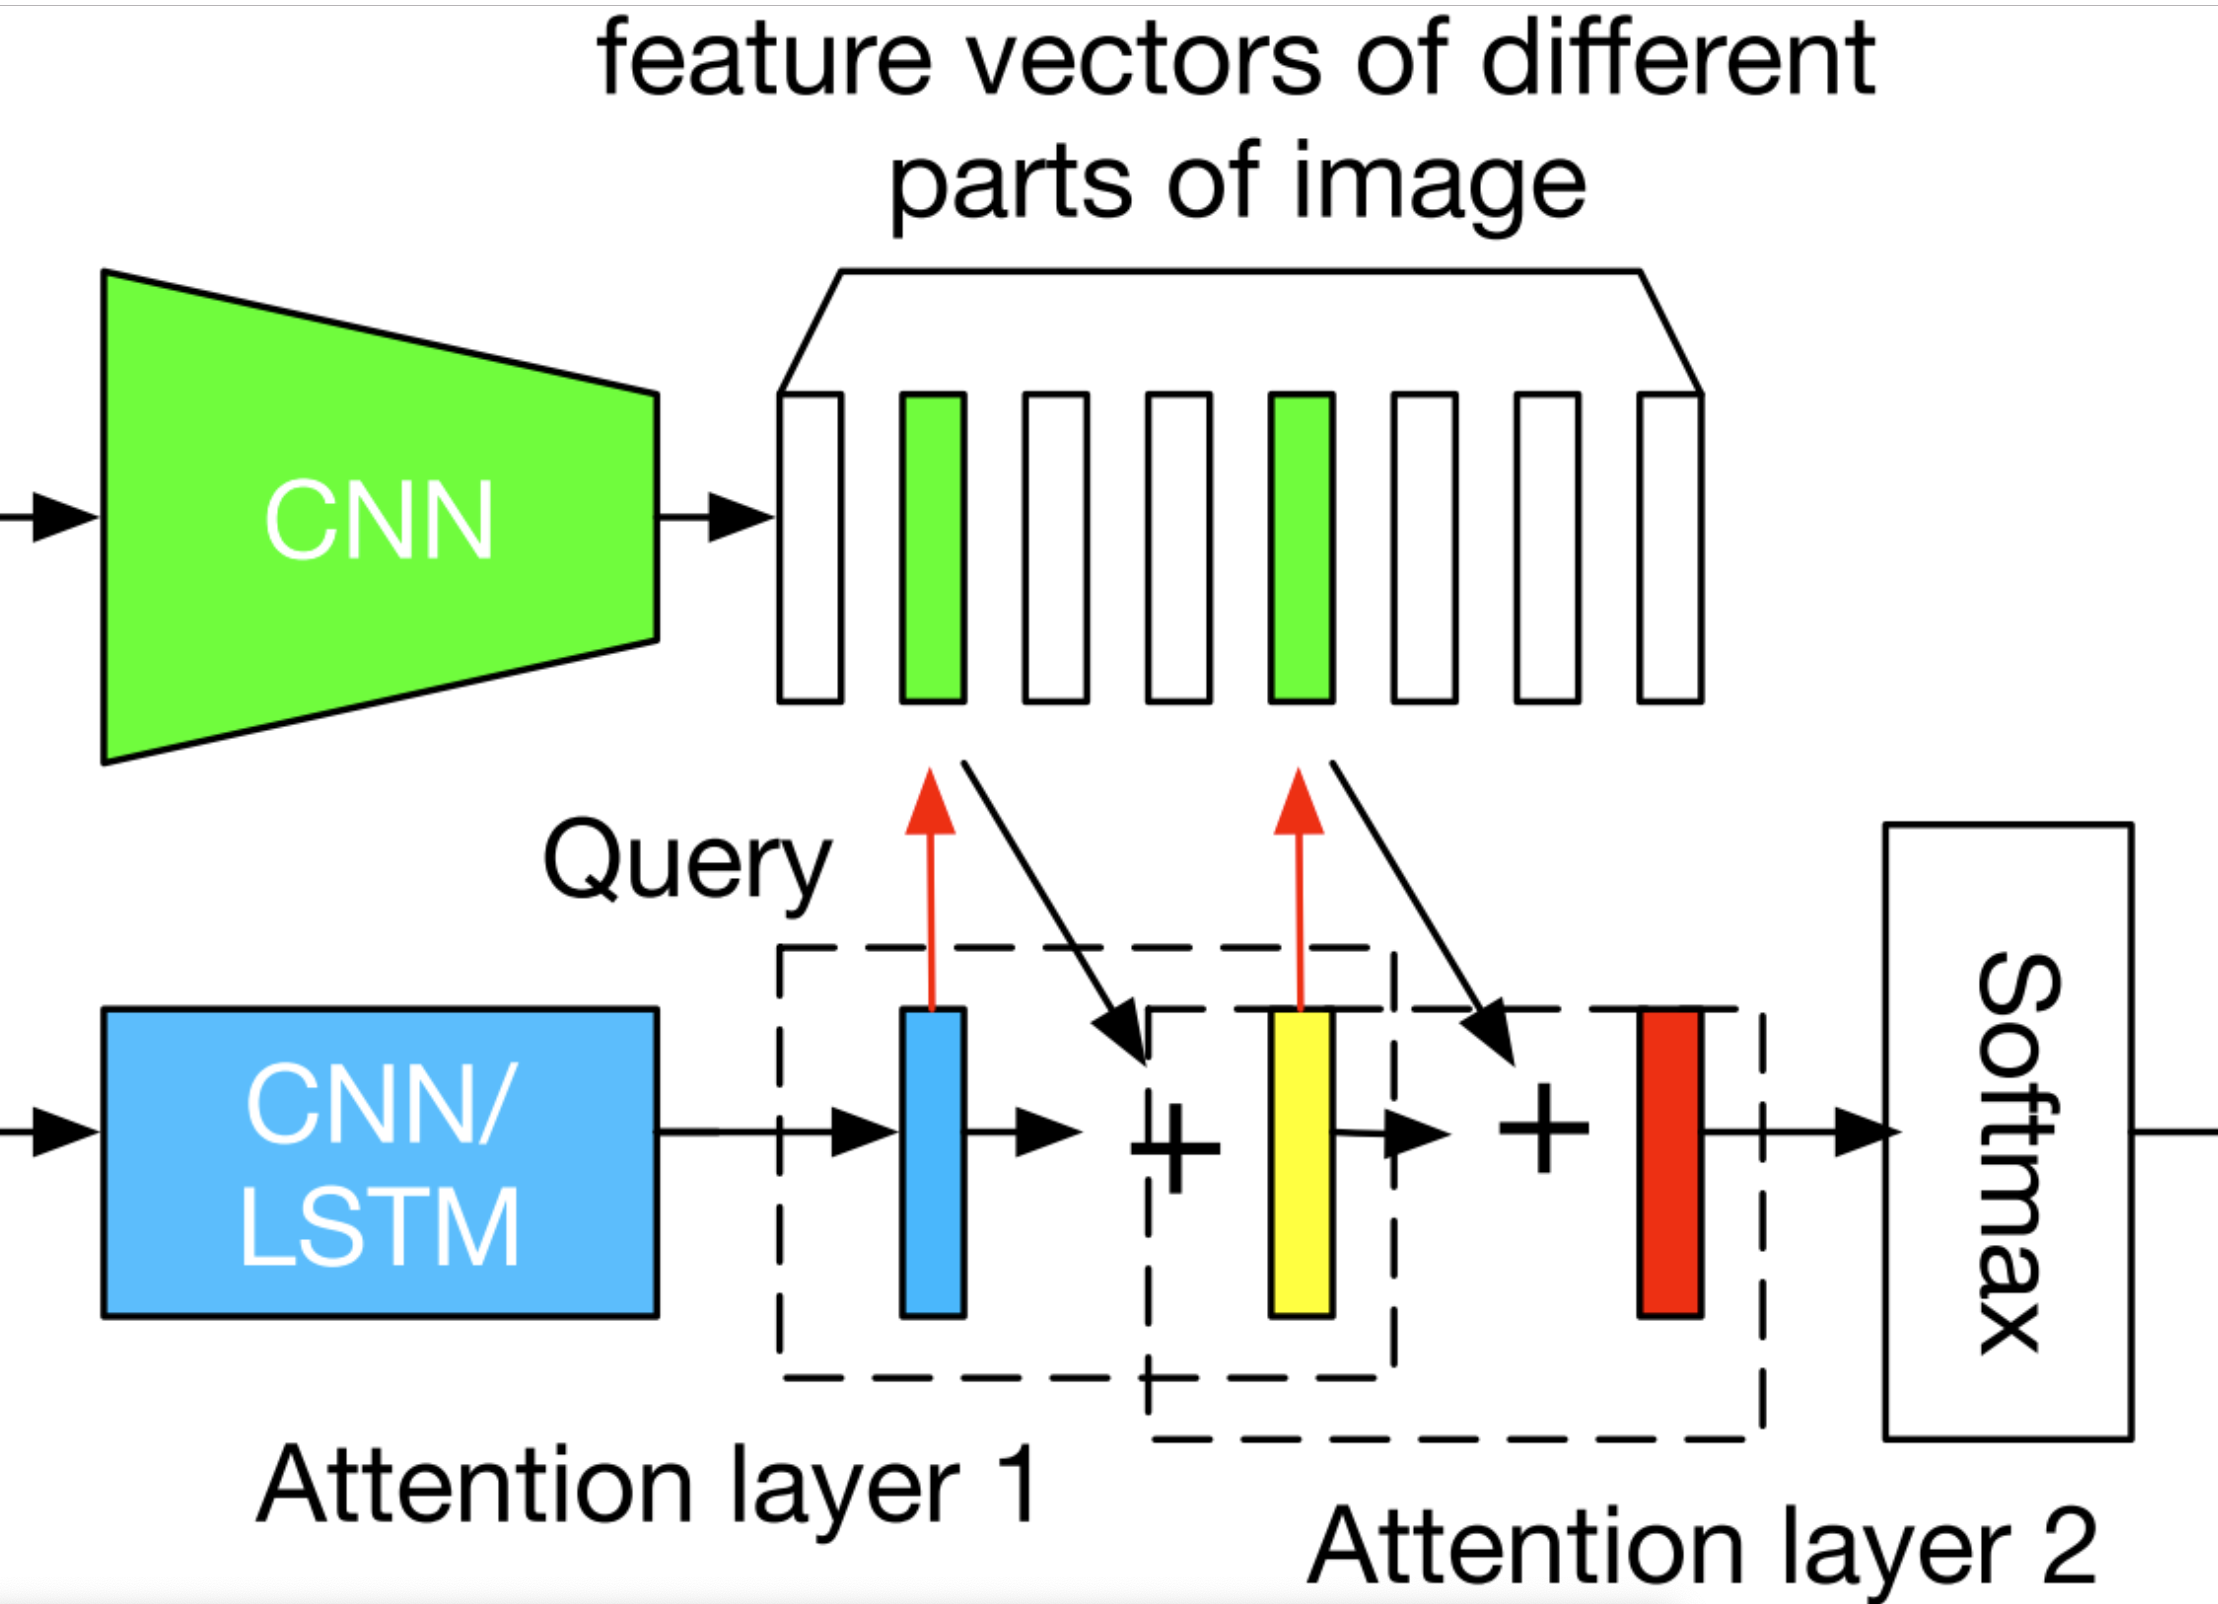
\includegraphics[scale = 0.55, width=8.5cm]{diagram_network.png}
\end{figure}
\vspace{-5mm}
We tried hyperparameter tuning, grid searching through them and chose to use the following parameters as they worked best for our dataset.
% \vspace{-5mm}
\begin{table}[!hbt]
		% Center the table
		\begin{center}
		% Title of the table
		\caption{Model Parameters}
		\label{tab:simParameters}
		% Table itself: here we have two columns which are centered and have lines to the left, right and in the middle: |c|c|
		\begin{tabular}{|c|c|}
			% To create a horizontal line, type \hline
			\hline
			% To end a column type &
			% For a linebreak type \\
			Batch Size & $256$ \\
			\hline
			Learning Rate & $0.001$ \\
			\hline
			Number of Iterations & $800$ \\
			\hline
			Number of Attention Layers & $2$\\
			\hline
			Word Embedding Size & $200$\\
			\hline
		\end{tabular}
		\end{center}
	\end{table}
\vspace{-5mm}
\section{Results}
    In order to evaluate our VQA Model we used the battle scenes dataset we built, which has 1511 battle scene images, with 31,731 QA pairs. This was split into 70-30 for train-test. When we applied our best VQA Model with model parameters as described in \textit{Section IV}, we got an \textbf{accuracy of 65.9\%} after 800 iterations. This accuracy was calculated with strict equivalence of answers and no points were given if the answer was even nearly correct, making our accuracy score strict and even a low accuracy score means, better results than the normal VQA Models. Refer Fig. 11 for the some of the best results our VQA Model produced, and Fig. 12 for some of the best and not-so-perfect yet meaningful results our model produced. Our model outputs completely meaningless results only in very rare cases. 
    
    \begin{figure}[ht]
        \caption{Best VQA Results (All Perfect)}
    \centering
     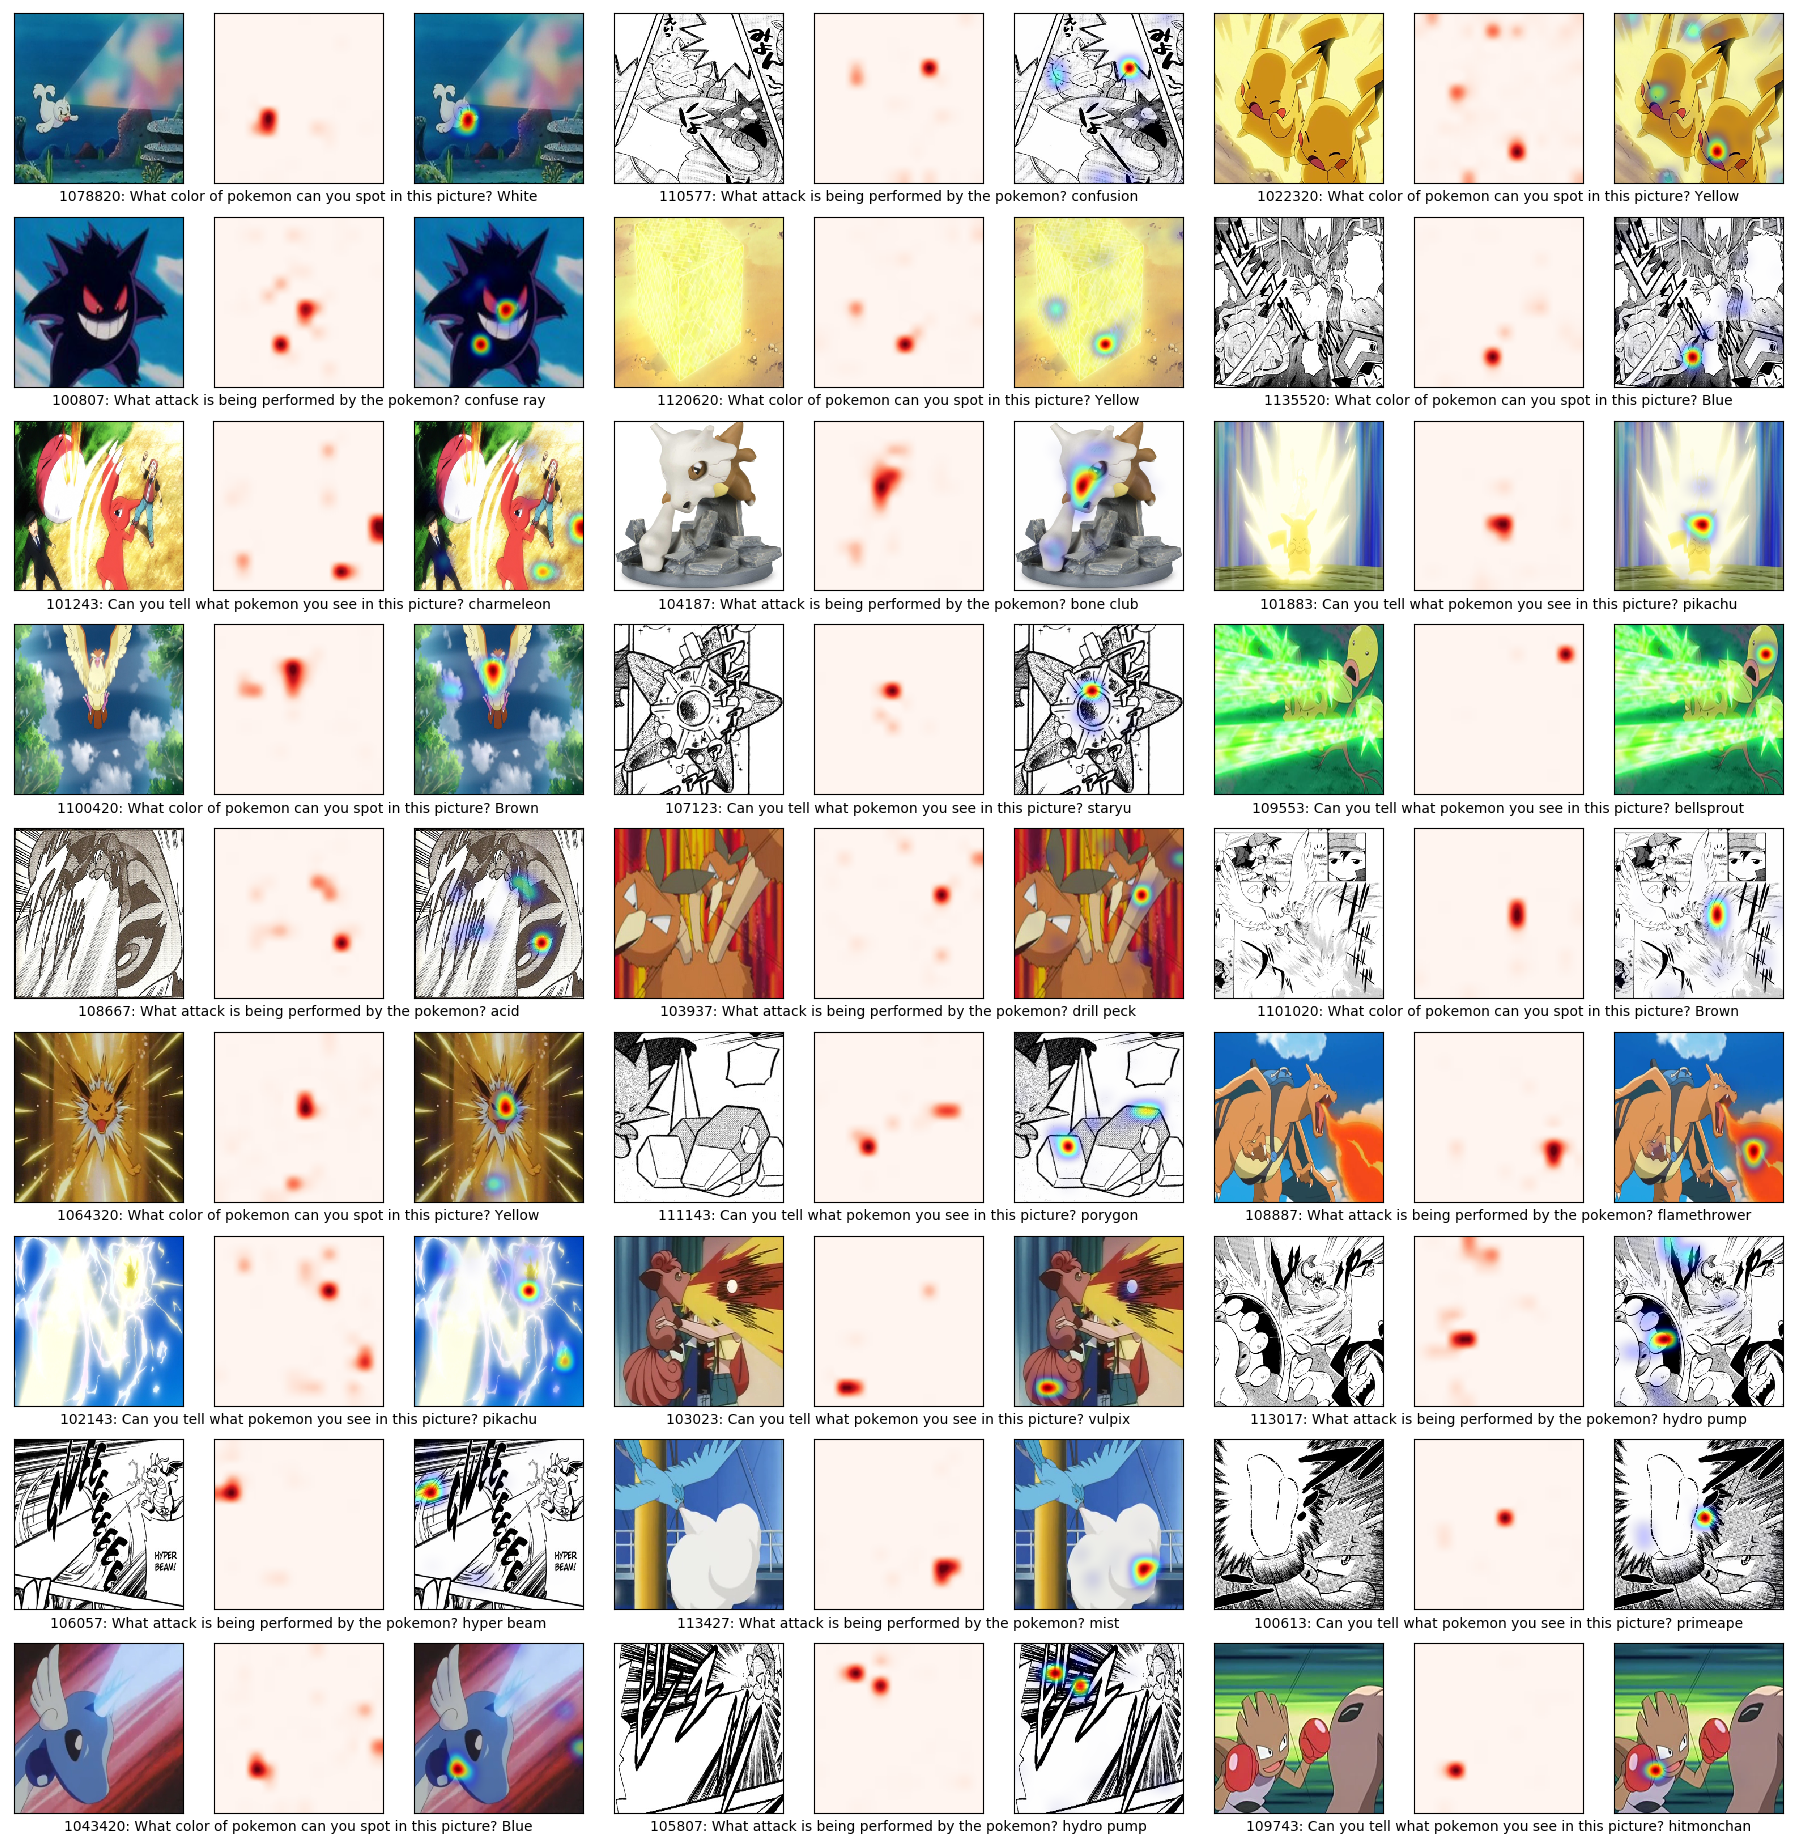
\includegraphics[scale = 0.6, width=9cm]{results_9x9_0_best.png}
    \end{figure}
    \begin{figure}[ht]
        \caption{Best VQA Results (Not so Perfect yet Meaningful)}
    \centering
     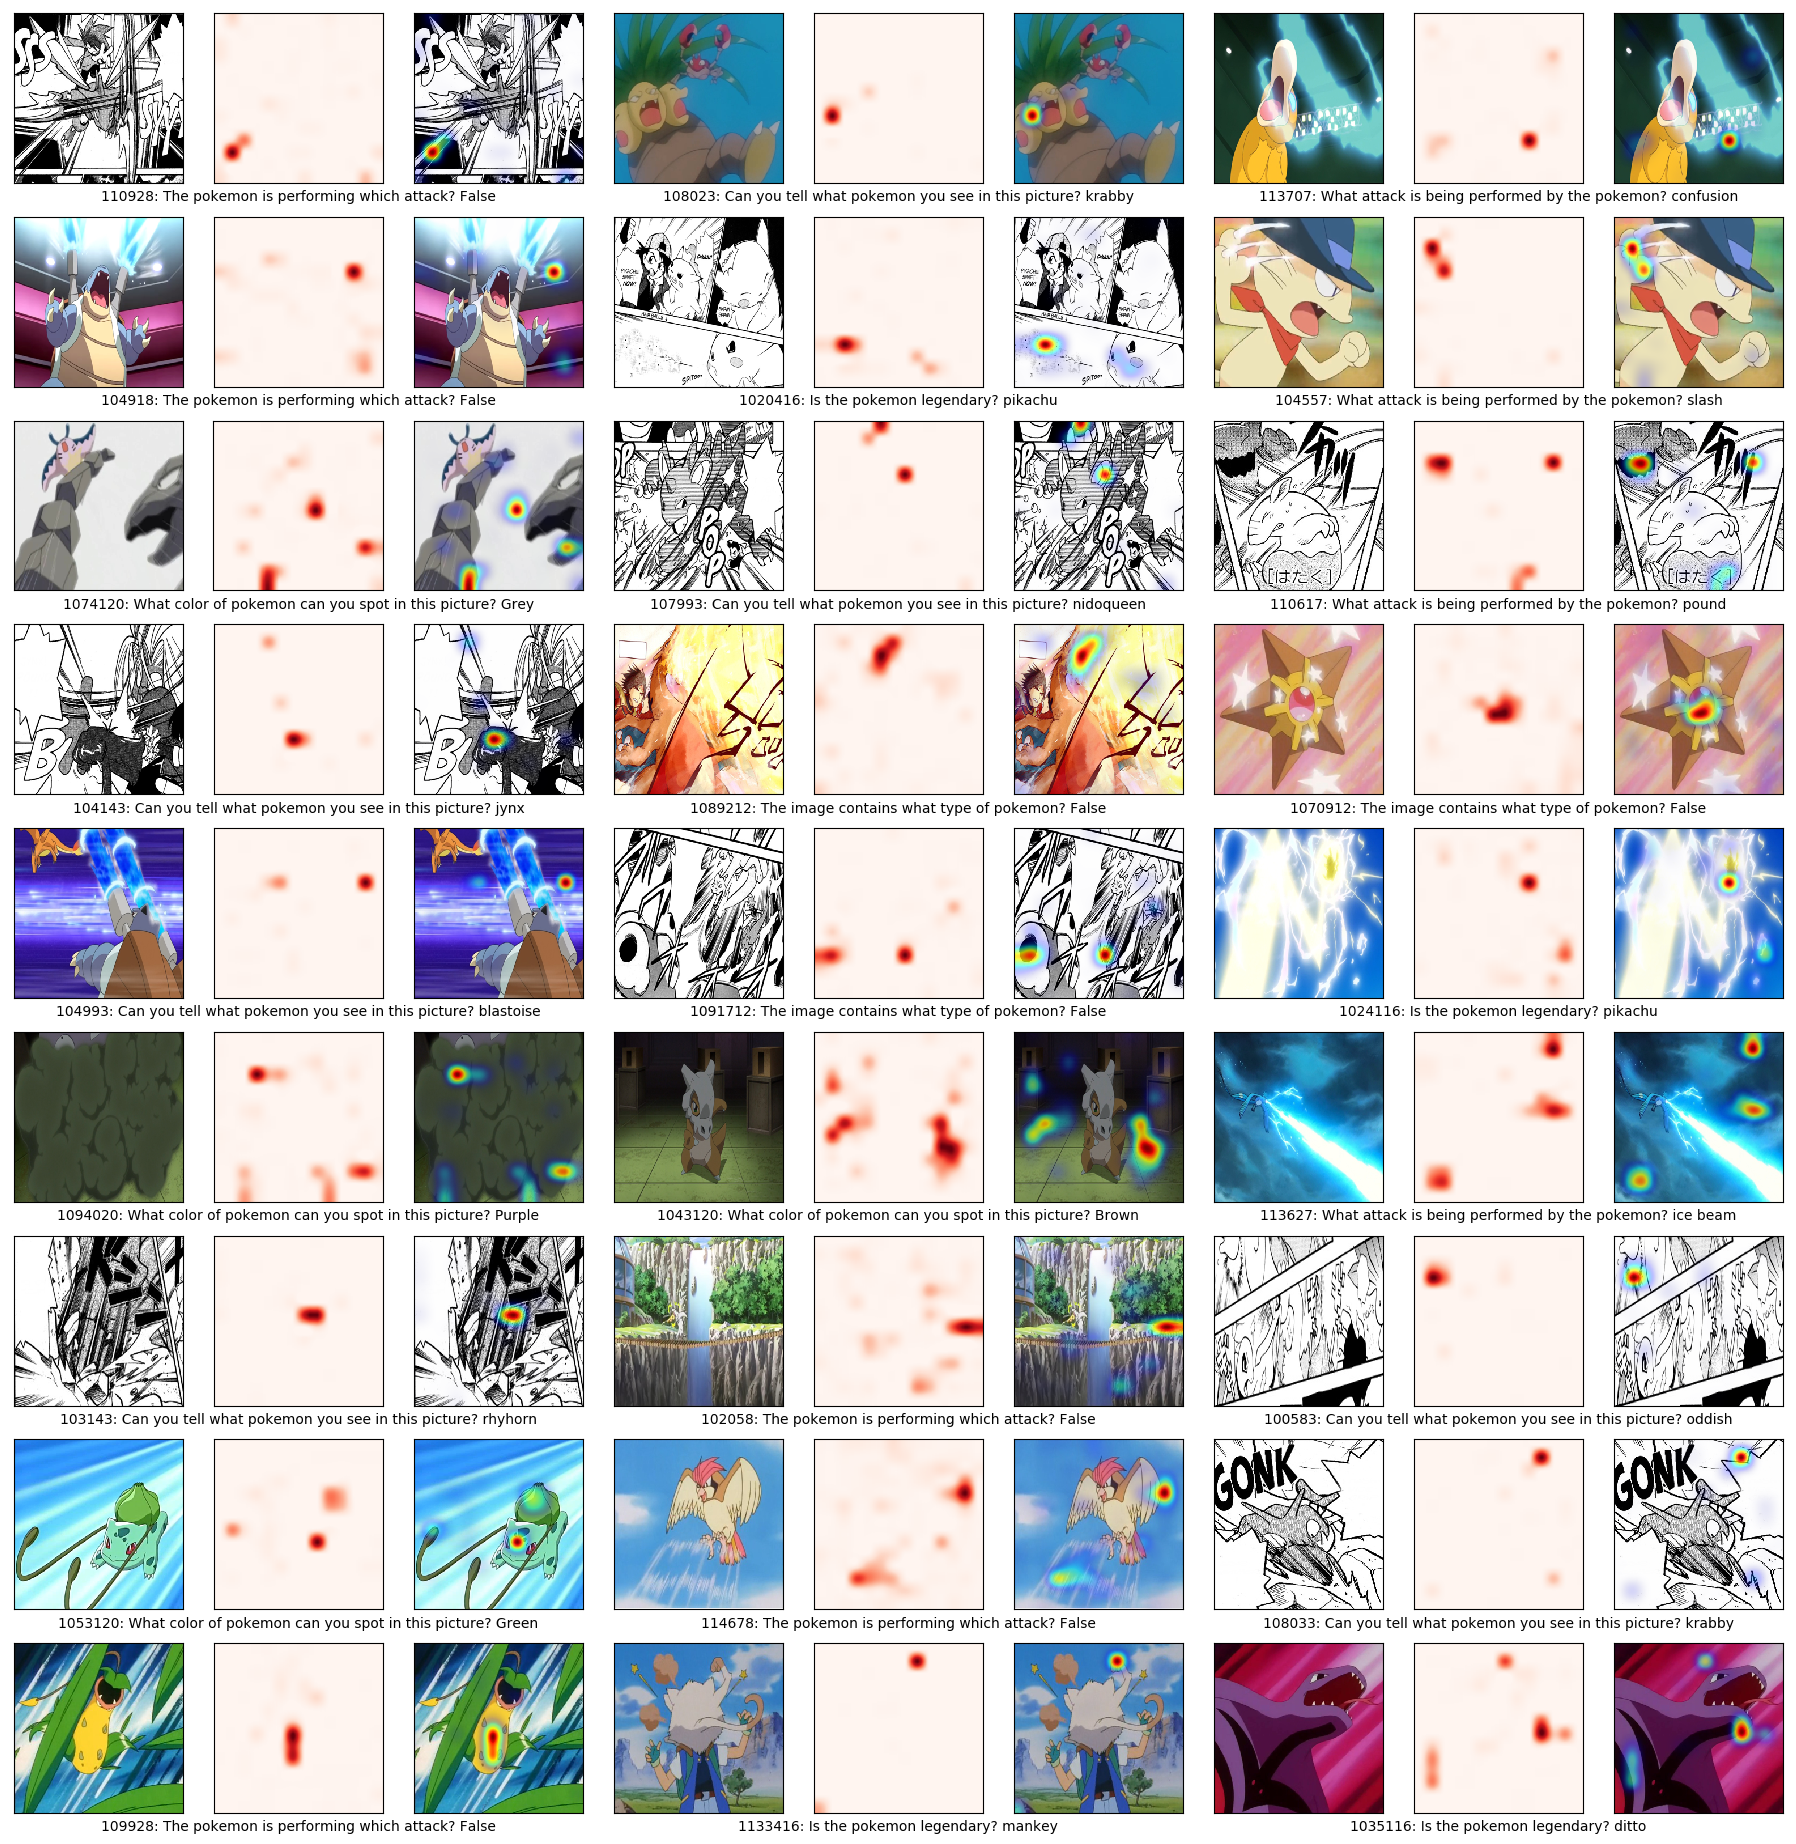
\includegraphics[scale = 0.6, width=9cm]{results_9x9_0_avg.png}
    \end{figure}
    
   Fig. 13 plots the change in Training loss with the number of iterations the network is trained. We see that as the training progresses, the curve undergoes a smooth decrease finally  saturating at 800 iterations. Hence our model learns well.
    
    \begin{figure}[ht]
        % \caption{Best VQA Results (Perfect and Nearly Perfect)}
    \centering
     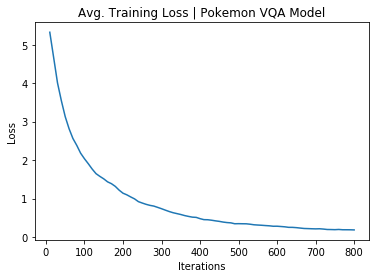
\includegraphics[scale = 0.6, width=9cm]{train_loss_curve.png}
    \end{figure}
    % \vspace{-5mm}
    % try to fit this in so that half a column remains of the 5th page after this
    
	% - our results (images - heatmaps and final outputs, also mention the accuracy and the number of images and questions used in the training/testing split)
	
	% - training/validation curves from the logs (from the train log file)
% 	\vspace{-5mm}
	 % (just mention how the same network on MSCOCO gets the similar result too and so we do well)
	From the results obtained on baseline datasets (as discussed in \cite{VQA_MODEL}), we can see that the performance of the VQA network on our dataset is good. VQA network gave an accuracy of 63.82\% on MSCOCO which is comparable to our 65.9\% In fact the network performs surprisingly well on the Pok\'emon dataset taking into account that our images are very bright, filled with fire/water/grass type Pokemons which are scattered across the images and are not localized. Also unlike MSCOCO, our dataset has lesser number of discriminative objects in its images. Hence intuitively, we had perceived this to be a harder problem as compared to benchmark datasets, but the VQA model outperformed our expectations.   
	
	%- Explain results
	On analyzing some specific results we get a sense of how robust the model is. For instance, let us consider questions 108887 (6th Row, 3rd Column, Fig. 11) and 113427 (8th Row, 2nd Column, Fig. 11), both of them are "What Attack?" questions and the model perfectly predicts "Flamethrower" and "Mist" respectively. What makes it more interesting is the fact that, it attends to/focuses at the correct place in the image to arrive at this answer. Proving that our answers are not just random and that the model makes sensible decisions. For example, in the first case it attends to the fire breath of Charizard and in the second case it attends to the cloud of mist from Articuno's mouth to answer the questions. The next interesting case is question 102143 (7th Row, 1st Column, Fig. 11), where we ask the model, what Pok\'emon it sees in the image, it perfectly focuses on the very small part of the image where is sees the Pikachu which is almost fully occluded by the Thuderbolt it produced and suggests that it was Pikachu, which is really interesting. Another question which really surprised us, was question 1135520 (2nd Row, 3rd Column, Fig. 11), where we have black and white image of Articuno performing an attack and the question was a "What Pokemon Color?" type question and to our surprise the model predicted perfectly that the color was Blue, which means that model first figured our that the Pok\'emon was Articuno and then it inferred from this fact that the color was Blue! Let us analyze one last image where the model predicted wrong, but did predicted a nearly perfect answer instead. See question 1020416 (2nd Row, 2nd Column, Fig. 12), where the question is "Is the Pok\'emon legendary?" and as the model does not know the correct answer for this question with high confidence it predicts Pikachu as the output, which is actually the answer to the "What Pok\'emon?" question, which is really sensible.
	
	Hence, the Pok\'emon VQA network is so robust and universal that it not only performs well to a specific dataset (MSCOCO) but also performs exceedingly well on our Pok\'emon dataset whose images are so obstructed and random. This is a huge step forward in research of VQA as we are literally able to answer questions about all kinds of images, thus helping us answer a broad spectrum of images. 

\section{Discussion}
    As can be seen above, we received positive results for the tough domain transfer in the VQA problem. We learned that VQA helps us to answer questions pertaining to all kinds of images, making it a highly useful tool. As a future problem, with additional compute resources and time available, we would like to attempt the transfer for Pok\'emon scene images having multiple pok\'emons and even trainers present in the image. As of now we had the another limitation of constraining our number of questions due to less visual content in the image. One of the advanced topics we look forward to working on involves predicting the outcome of a battle by looking at the battle stage in the image and some additional prior about the Pok\'emon weaknesses and strengths.
    
Also, due to the less visual content in our images, we could only form questions having a fixed answer, though in real world (in the poke\'mon world too!) there can be multiple correct answers to a single question. For that we came across \cite{GURARI} which deals with automatically predicting from a visual question whether a
crowd would agree on one answer or not. It also proposes how to
exploit these predictions to efficiently collect all valid answers to visual questions. 

Through this course we learned to leverage the power of deep learning models to solve problems on large datasets efficiently and accurately. We also learned to reason about why our changes to the models work and the possible intuition of the mathematics behind it. As experienced deep learning students, we would now imagine looking at every paper or model we come across with a mathematical and logical bend about their working.

We highly recommend this course to all students as it introduced us to all the current Deep Learning techniques being used in the real world. We believe that knowledge of these techniques is crucial to our understand of how everything that surrounds us is being predicted/classified, in this era of digitization. For a student, taking this course would not only mean that you need to understand the mathematics behind the algorithms involved but would also require you to experiment with the parameters involved in these algorithms, in order to understand how these parameters are controlling the behaviour of the algorithms. The course will keep you busy in optimising your results as well as analysing why you are getting a particular result. We appreciate the efforts put in by the instructors including the professor and the TAs. 
% Now we need a bibliography:
\begin{thebibliography}{5}

	%Each item starts with a \bibitem{reference} command and the details thereafter.
	\bibitem{PYTHIA}
	Jiang, Yu, Vivek Natarajan, Xinlei Chen, Marcus Rohrbach, Dhruv Batra, and Devi Parikh. "Pythia v0. 1: The winning entry to the vqa challenge 2018." arXiv preprint arXiv:1807.09956 (2018).
	
	\bibitem{BOTTOMUP}
	Anderson, Peter, Xiaodong He, Chris Buehler, Damien Teney, Mark Johnson, Stephen Gould, and Lei Zhang. "Bottom-up and top-down attention for image captioning and visual question answering." In CVPR, vol. 3, no. 5, p. 6. 2018.
	
	\bibitem{VQA1}
	\url{https://github.com/iamaaditya/VQA_Keras}
	
	\bibitem{VQA2}
	\url{https://github.com/anantzoid/VQA-Keras-Visual-Question-Answering}
	
	\bibitem{SELECTIVE SEARCH}
	Uijlings, J.R.R., van de Sande, K.E.A., Gevers, T. et al. Int J Comput Vis (2013) 104: 154. https://doi.org/10.1007/s11263-013-0620-5
	
	\bibitem{SELECTIVE SEARCH CODE}
	\url{https://github.com/AlpacaDB/selectivesearch}
	
	\bibitem{googlenet}
	Christian Szegedy, Wei Liu, Yangqing Jia, Pierre Sermanet, Scott Reed, Dragomir Anguelov, Dumitru Erhan, Vincent Vanhoucke, Andrew Rabinovich; The IEEE Conference on Computer Vision and Pattern Recognition (CVPR), 2015, pp. 1-9
	
	\bibitem{IMAGENET}
	\url{http://www.image-net.org/}
	
	\bibitem{KAGGLE} % dataset link
	\url{https://www.kaggle.com/thedagger/pokemon-generation-one/discussion}
	\bibitem{BULBAPEDIA}
	\url{https://archives.bulbagarden.net/wiki/Special:ListFiles}
	
	\bibitem{MOVES}
	\url{https://www.kaggle.com/n2cholas/competitive-pokemon-dataset}
	\bibitem{STATS}
	\url{https://www.kaggle.com/rounakbanik/pokemon}
	
	\bibitem{MIT 205 PLACES}
	\url{http://places.csail.mit.edu/downloadCNN.html}
	
	\bibitem{WIKIA}
	\url{http://pokemon.wikia.com/wiki/Pok%C3%A9mon_Wiki}
    
    \bibitem{VQA_MODEL}
    \url{https://github.com/abhshkdz/neural-vqa-attention}
    
    \bibitem{GURARI}
    Danna Gurari and Kristen Grauman. 2017. CrowdVerge: Predicting If People Will Agree on the Answer to a Visual Question. In Proceedings of the 2017 CHI Conference on Human Factors in Computing Systems (CHI '17). ACM, New York, NY, USA, 3511-3522. DOI: https://doi.org/10.1145/3025453.3025781
	
	

\end{thebibliography}

% Your document ends here!
\end{document}